\documentclass[a4paper]{article}

\usepackage[T1]{fontenc}
\usepackage[adobe-utopia]{mathdesign}
\usepackage[protrusion=true,expansion=true]{microtype}
\usepackage{xcolor}
\usepackage{graphicx}

\definecolor{darkblue}{rgb}{0,0,0.5}

\usepackage[colorlinks=true,
        urlcolor=darkblue,
        anchorcolor=darkblue,
        linkcolor=darkblue,
        citecolor=darkblue,
        pdfauthor={Mohannad Banayosi},
        pdfkeywords={educational tools, pseudo-code, virtual machine,
          parser, interpreter},
        pdftitle={Real-time fitness monitor.},
        pdfsubject={Real-time fitness monitor,
          the German University in Cairo GUC
          (http://met.guc.edu.eg/)}]{hyperref}
\usepackage{url}

\author{Mohannad Banayosi}
\title{Real-time fitness monitor.}

\begin{document}

\maketitle

\begin{abstract}
IMPACT is a multidisciplinary project in which students of computer science (more precisely: software engineering), material sciences, mechatronics and embedded system design come together to create Thai-boxing pads with builtin impact sensors and wireless connection to a base station.
In this project, we will implement a multi-sensor tracking and analysis tool for a physical workout routine specific to Thai/kick-boxing or similar contact sports to track and display performance and fitness level of a practitioner over a single and over multiple sessions. It will be used to record and correlate the inputs from impact sensors and technique recognition and track improvemets of practitioners over time.
  
\end{abstract}

\newpage

\section{Introduction}
\begin{figure}[h!]
\centering
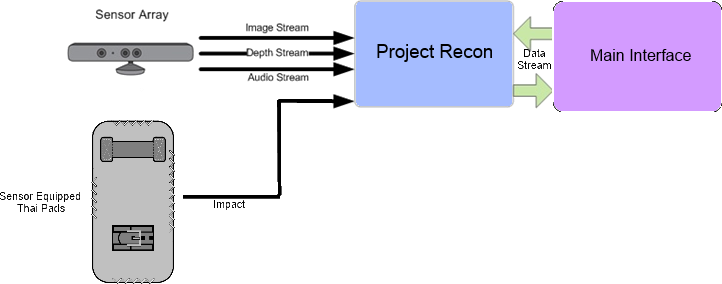
\includegraphics[scale=0.6]{General.png}
\caption{General Overview}
\label{threadsVsSync}
\end{figure}

\subsection{Problem}
In the world of martial arts, there is no accurate way to study and analyze the performance of the trainee. This absence of analysis is due to the lack of tools presented to the trainers.

\subsection{Aim of this project}
The aim of this project is to deliver an easy-to-use interface that displays training sessions' info and statistics. This in turn will help the trainers to get an accurate analysis of the trainee's performance.

\section{Technologies and frameworks}
A lot of technologies and frameworks have been researched, some of them were chosen to be used and others not. Following is a list of them.

\subsection{Not used}
Most of the technologies researched where not used because of their violation of the core feature of the interface being generic.

\subsubsection{Depthjs}
Depthjs was developed by four MIT students, Aaron Zinman, Doug Fritz, Greg Elliott and Roy Shilkrot in 2010. Depthjs allows any web page to interact with the Microsoft Kinect using Javascript. It provides the low-level raw access to the Kinect as well as high-level hand gesture events to simplify development.
\\* Depthjs is an open source project, but with no enough documentation, compatible with Google chrome only, and is more helpful in web navigation.

\subsubsection{Zigfu}
Zigfu was developed by Ted Blackman, Shlomo Zippel, Roee Shenberg, Amir Hirsch, Bryce Tucker. They developed the ZDK (Zigfu Development Kit) to make cross-platform, motion-controlled apps with Kinect in HTML5/Javascript, Unity3D and Flash. Applications made with this development kit are portable across all operating systems, web browsers, computer vision middlewares, and 3D sensors. 
\\*Zigfu is not an open source project, still have problems in performance and accuracy in gesture recognition.


\subsubsection{OpenDepth}
OpenDepth - Extending the Web - is a client server application developed by Ecaterina Paun, Narcis Paun and Mircea Piturca. OpenDepth brings Kinect SDK methods and data to the web with the server side written on C\# and built on top of Kinect SDK 1.5, while the client side is a written in JavaScript and uses the Three.js webGL rendering engine.
\\* It is an open source project, with enough documentation, and is more helpful in web navigation.

\subsection{Used}
*Few words here*

\subsubsection{Django}
Django is a high-level Python Web framework that encourages rapid development and clean, pragmatic design. Developed by a fast-moving online-news operation, Django was designed to handle two challenges: the intensive deadlines of a newsroom and the stringent requirements of the experienced Web developers who wrote it. It lets you build high-performing, elegant Web applications quickly.

\subsubsection{Web Sockets}
*Advantages*
\\**Disadvantages*
\\**Why I will use it*

\section{The interface}
You will implement a multi-sensor tracking and analysis tool for a specific physical workout routine to track performance and fitness level of a practitioner over a single and over multiple sessions.

This interface should have the capability to get several plugins connected to it.

\subsection{Architecture}
The following architecture's design represents the different components included in the interface.
\newpage

\begin{figure}[h!]
\centering
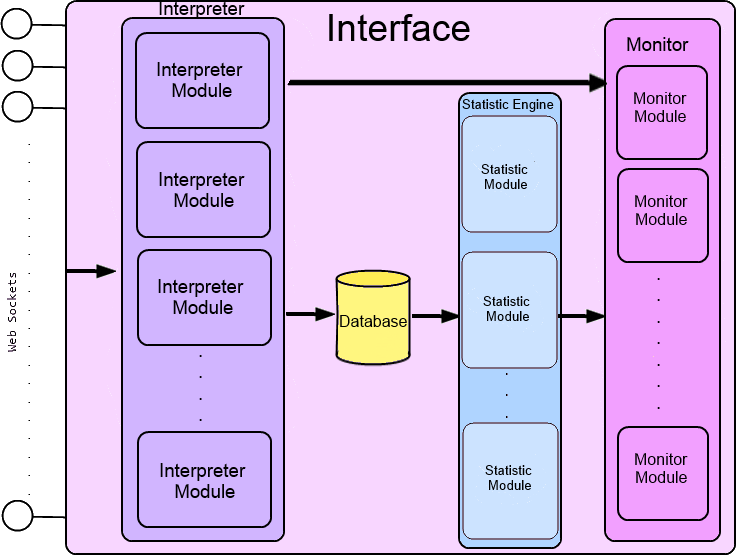
\includegraphics[scale=0.6]{Interface.png}
\caption{The Architecture}
\label{threadsVsSync}
\end{figure}

\subsubsection{Interpreter}
Containing several interpreter modules, the interpreter serves as the brain of the interface receiving the data (initially received through the sockets) and then begins digesting and translating it into actual info. It then sends it to the monitor (to display the data received) and the database manager (to save the data).

\begin{figure}[h!]
\centering
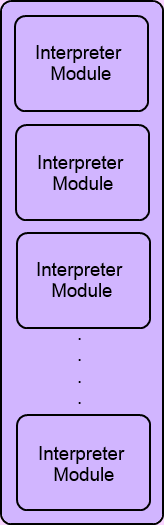
\includegraphics[height=60mm]{Interpreter.png}
\caption{The Interpreter}
\label{threadsVsSync}
\end{figure}

\subsubsection{Database engine}
The database engine saves the users and their data; this data, or history, is collected from previous sessions the trainee took.

\subsubsection{Statistics engine}
Containing several statistics modules, this engine generates the analysis (this analysis depends on the current data received + the history of the trainee) and sends it to the monitor.

\begin{figure}[h!]
\centering
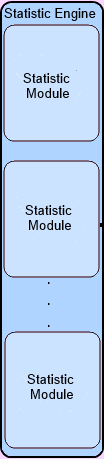
\includegraphics[height=60mm]{Statistics.png}
\caption{The Statistics Engine}
\label{threadsVsSync}
\end{figure}

\subsubsection{Monitor}
The monitor is the front end component of the interface that displays all the info (including live data and statistics-related data). It contains several monitoring modules together make up the monitor.

\begin{figure}[h!]
\centering
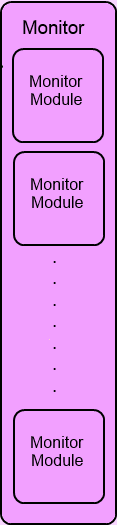
\includegraphics[height=55mm]{Monitor.png}
\caption{The Monitoring System}
\label{threadsVsSync}
\end{figure}

\subsection{Hand shaking}
This is the process where each plugin reserves a web socket to start the data stream with the interface. This begins when the plugin sends a request to the interface via a socket, then the interface reserves the socket for the plugin and sends an OK signal. Once the OK signal is received, the plugin can start the data stream at any time.

\subsection{Data stream}
The data stream contains the type of the data sent (on-session or off-session), a timestamp and the actual data.

\end{document}

%%% Local Variables: 
%%% mode: latex
%%% TeX-master: t
%%% End: 